\documentclass[12pt]{article}
\usepackage{graphicx}

\pagestyle{empty}
\setcounter{secnumdepth}{2}

\topmargin=0cm
\oddsidemargin=0cm
\textheight=22.0cm
\textwidth=16cm
\parindent=0cm
\parskip=0.15cm
\topskip=0truecm
\raggedbottom
\abovedisplayskip=3mm
\belowdisplayskip=3mm
\abovedisplayshortskip=0mm
\belowdisplayshortskip=2mm
\normalbaselineskip=12pt
\normalbaselines

\begin{document}

\vspace*{0.5in}
\centerline{\bf\Large Design Document}

\vspace*{0.5in}
\centerline{\bf\Large Team 3}

\vspace*{0.5in}
\centerline{\bf\Large 11 March 2012}

\vspace*{1.5in}
\begin{table}[htbp]
\caption{Team}
\begin{center}
\begin{tabular}{|r | c|}
\hline
Name & ID Number \\
\hline\hline
John Alexander Landovskis & 9641394\\
Eric Regnier & 9332219\\
Rahmat Jaffari & 9095926\\
Bacacar Ndiaye & 9744258\\
Kam Shing Yip & 9602518\\
X & Y\\
X & Y\\
X & Y\\
X & Y\\
\hline
\end{tabular}
\end{center}
\end{table}

\clearpage

\section{Introduction}

The introduction of the document provides an overview of the entire document,
briefly introducing what are its goals, and what information is to be found in it.

\section{Architectural Design} \label{sec:arch}

This section must give a high-level description of the system in terms of its modules
and their respective purpose and exact interfaces.

\subsection{Architectural Diagram}
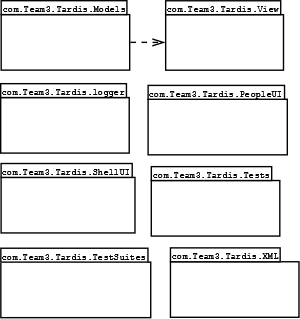
\includegraphics{diagrams/package_diagram}
\\
A UML class diagram or package diagram depicting the high-level structure of the system,
accompanied by a one-paragraph text describing the rationale of this design.
It is mandatory that the system be divided into at least two subsystems,
and that the purpose of each of these subsystems be exposed here.

\subsection{Subsystem Interface Specifications}

Specification of the software interfaces between the subsystems,
i.e. specific messages (or function calls) that are exchanged by the subsystems.
These are also often called ``Module Interface Specifications''.
Description of the parameters to be passed into these function calls in order to have a service fulfilled,
including valid and invalid ranges of values.
Each subsystem interface must be presented in a separate subsection.


\section{Detailed Design} \label{sec:detail}

Complete description of the system design, describing one subsystem separately in respective subsection.
UML class diagrams are to be used, as well as a short textual description describing the purpose of each class.

\subsection{Subsystem $<$Models$>$}

\subsubsection{Detailed Design Diagram}

UML class diagram depicting the internal structure of the subsystem,
accompanied by a paragraph of text describing the rationale of this design.

\subsubsection{Units Description}

List each class in this subsystem and write a short description of its purpose,
as well as notes or reminders useful for the programmers who will implement them.
List all attributes and functions of the class.
\subsection{Subsystem $<$Controller$>$}

\subsubsection{Detailed Design Diagram}
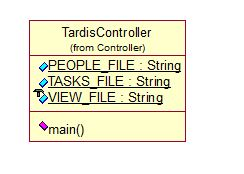
\includegraphics{subsystems/diagrams/controller_class_diagram.jpg}

UML class diagram depicting the internal structure of the subsystem,
accompanied by a paragraph of text describing the rationale of this design.

The controller is resposible for loading the data and giving it to the view.

\subsubsection{Units Description}

\emph{TardisController}\\
Functions:\\
\begin{tabular}{| l | l | l | l |}
\hline
Name & Parameters & Pre-conditions & Post-conditions\\
\hline
\multirow{2}{*}{main} & String[] args & Requires Nothing & Ensures that the data has been loaded\\ 
			 &  & & and passed to the main view
\\
\hline
\end{tabular}\\
\\
Attributes:\\
\begin{tabular}{| l | l |}
\hline
Name & Description\\
\hline
String PEOPLE\_FILE & The assumed name of the file containing the people.\\
\hline
String TASKS\_FILE & The assumed name of the file containing the tasks.\\
\hline
String VIEW\_FILE & The assumed name of the file in which to dump the people.\\
\hline 
\end{tabular}

Purpose: The main program. Loads the people and tasks from the files and passes them to the main view.

List each class in this subsystem and write a short description of its purpose,
as well as notes or reminders useful for the programmers who will implement them.
List all attributes and functions of the class.
\subsection{Subsystem $<$Views$>$}

\subsubsection{Detailed Design Diagram}
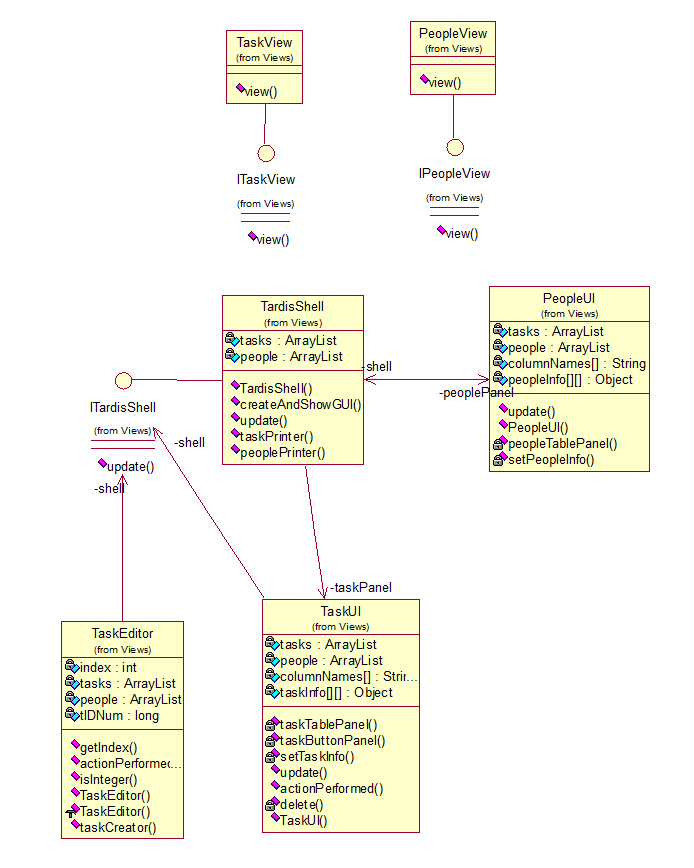
\includegraphics{subsystems/diagrams/views_class_diagram.png}

UML class diagram depicting the internal structure of the subsystem,
accompanied by a paragraph of text describing the rationale of this design.

The purpose of the views subsystem is to display the models cotained in the models subsystem. The idea was to seperate the application and presentation logic. This is used to meet the software engineering goal of loose coupling.

\subsubsection{Units Description}
\emph{PeopleUI}\\
Functions:\\
\begin{tabular}{| l | l | l | l |}
\hline
Name & Parameters & Pre-conditions & Post-conditions\\
\hline
\multirow{2}{*}{PeopleUI}{} & TardisShell shell & Requires Nothing & Ensures that\\ 
			        & ArrayList$<$Task$>$ tasks & & layout has been\\ 
                                            & ArrayList$<$Person$>$ peopleArray & &  setup.
\\
\hline
\multirow{2}{*}{void peopleTablePanel} & None & Requires Nothing & Ensures that\\
& & & the table view\\
& & & for people has\\
& & & been created.
\\
\hline
\multirow{2}{*}{void setPeopleInfo} & None & Requires a valid & Ensures that the\\
		 		            &          & list of people.     & people data is in\\
                                                            &         &                             & the table.
\\
\hline
\multirow{2}{*}{void update} & None & Requires a valid & Ensures that the\\
		                 &          & list of people.     & people data in the\\
		                 &          &                            & table is up to date.
\\
\hline
\end{tabular}\\
\\
Attributes:\\
\begin{tabular}{| l | l |}
\hline
Name & Description\\
\hline
TardisShell shell & The manager of the main view.\\
\hline
ArrayList$<$Task$>$ tasks & The tasks that the user created.\\
\hline
ArrayList$<$Person$>$ people & The people that can be assigned tasks.\\
\hline
String[] columnNames & The field names that will be displayed in the table.\\
\hline
Object[][] peopleInfo & The people in a generic format for the table.\\
\hline
JPanel peopleTablePanel & The panel containing the table.\\
\hline
JTable peopleTable & The table containing the people.\\
\hline
DefaultTableModel model & The generic model used by the JTable.\\
\hline
\end{tabular}

Purpose: Display the people as a table.\\
\\
\\
\emph{TaskUI}\\
Functions:\\
\begin{tabular}{| l | l | l | l |}
\hline
Name & Parameters & Pre-conditions & Post-conditions\\
\hline
\multirow{2}{*}{TaskUI}{} & ITardisShell shell & Requires Nothing & Ensures that the\\ 
			        & ArrayList$<$Task$>$ tasks & & task layout has been\\ 
                                            & ArrayList$<$Person$>$ people & & setup.
\\
\hline
\multirow{2}{*}{void actionPerformed} & ActionEvent e & Requires that e            & Ensures that\\
                                                                &                        & is a valid action event. & the button press\\
                                                                &                        &                                      & was interpreted.
\\
\hline
\multirow{2}{*}{void delete} & int row         & Requires that row points & Ensures that the task \\
		 	           &                     & to an existing row.          & and its subtasks\\
		 	           &                     &                                         & were deleted.\\
 			           &                     &                                         & Ensures that the task\\
                                               &                     &                                         & view was updated.
\\
\hline
\multirow{2}{*}{void setTaskInfo} & None & Requires a valid list & Ensures that the task \\
		 		        &          & of tasks.                   & data is in the table. 
\\
\hline
\multirow{2}{*}{void update} & None & Requires a valid list & Ensures that the task\\
		 	             &          & of tasks.                  & data in the table is\\
			             &          &                                 & up to date.
\\
\hline
\multirow{2}{*}{void taskButtonPanel} & None & Requires Nothing & Ensures that the\\
		 	                            &          &                             & add, edit and delete\\
                                                                &          &                             & buttons have been\\
					    &          &                             & created.
\\
\hline
\multirow{2}{*}{void taskTablePanel} & None & Requires Nothing & Ensures that the\\
		 	                         &           &                             & table view was\\
				             &           &                             & created.
\\
\hline
\end{tabular}

Attributes:\\
\begin{tabular}{| l | l |}
\hline
Name & Description\\
\hline
String[] columnNames & The field names that will be displayed in the table.\\
\hline
DefaultTableModel model & The generic model used by the JTable.\\
\hline
ArrayList$<$Person$>$ people & The people that can be assigned tasks.\\
\hline
ITardisShell shell & The manager of the main view.\\
\hline
JPanel taskButtonPanel & The panel containing the add, edit and delete buttons.\\
\hline
Object[][] taskInfo & The tasks in a generic format for the table.\\
\hline
ArrayList$<$Task$>$ tasks & The tasks that the user created.\\
\hline
JTable taskTable & The table containing the tasks.\\
\hline
JPanel taskTablePanel & The panel containing the tasks table.\\
\hline
\end{tabular}\\
\\
Purpose: Display the tasks as a table.\\
\\
\\
\emph{TaskEditor}\\
Functions:\\
\begin{tabular}{| l | l | l | l |}
\hline
Name & Parameters & Pre-conditions & Post-conditions\\
\hline
\multirow{2}{*}{TaskEditor} & ITardisShell shell                         & Requires Nothing & Ensures that the task\\ 
			          & ArrayList$<$Task$>$ tasks       &                             & editor has been created.\\ 
                                              & ArrayList$<$Person$>$ people &                             & 
\\
\hline
\multirow{2}{*}{TaskEditor} & ITardisShell shell                         & Requires Nothing & Ensures that the task\\ 
			          & ArrayList$<$Task$>$ tasks       &                             & editor has been created\\ 
                                              & ArrayList$<$Person$>$ people &                             & and populated with\\
			          & int index                                      &                            & the data of the\\
			          &                                                     &                            & selected element.
\\
\hline
\multirow{2}{*}{void actionPerformed} & ActionEvent e & Requires that e            & Ensures that\\
                                                        &                        & is a valid action event. & the button press\\
                                                        &                        &                                      & was interpreted.
\\
\hline
\multirow{2}{*}{bool isInteger} & String in & Requires Nothing & Ensures that the\\
		 	                &               &                             & input is a valid\\
		 	                &               &                             & integer.
\\
\hline
\multirow{2}{*}{void taskCreator} & long taskId                    & Requires Nothing & Ensures that either\\
		 	             & String title                     &                             & a new task was created\\
                                                 & String shortDescription &                             & or an existing task\\
				 & int duration                   &                             & was modified.\\
				 & String deliverable          &                             &\\
		       		 & Date dueDate               &                             &\\
				 & int personID                  &                             &\\
				 & Task parent                   &                             &
\\
\hline
\multirow{2}{*}{void updateTask} & None & Requires Nothing & Ensures that the task\\
		                               &           &                             & has been modified.
\\
\hline
\multirow{2}{*}{bool validateDate} & None & Requires Nothing & Ensures that the date\\
		                                  &           &                            & is valid. 
\\
\hline
\multirow{2}{*}{bool validateDuration} & None & Requires Nothing & Ensures that the\\
		                                        &           &                            & duration is valid.
\\
\hline
\multirow{2}{*}{bool validateTitle} & None & Requires Nothing & Ensures that the title\\
		                                &           &                             & is valid.
\\
\hline
\end{tabular}

Attributes:\\
\begin{tabular}{| l | l |}
\hline
JButton CANCEL & The button to close the task window without making changes.\\
\hline
JComboBox cPeople & The control to select who the task is assigned to.\\
\hline
JComboBox cSuper & The control to select the super task.\\
\hline
JLabel cSuperL & The label containing the supertask description.\\
\hline
JLabel deliverable & The label containing the deliverable description.\\
\hline
JLabel dueDateD & The label containing the description of the day part of the due date.\\
\hline
JLabel dueDateM & The label containing the description of the month part of the due date.\\
\hline
JLabel dueDateY & The label containing the description of the year part of the due date.\\
\hline
JLabel duration & The label containing the description of the duration.\\
\hline
int index & The position in the list of tasks.\\
\hline
JPanel panel & The panel containing the task controls.\\
\hline
ArrayList$<$Person$>$ people & The people that can be assigned tasks.\\
\hline
JLabel personID & The description of the person id.\\
\hline
ITardisShell shell & The manager of the main view.\\
\hline
JLabel shortDesc & The description of the short description.\\
\hline
\multirow{2}{*}{JButton SUBMIT} & The button to save a new task or\\
				       & the modifications made to an existing task.
\\
\hline
JLabel superID & The label containing the supertask id.\\
\hline
JLabel taskID & The label containing the description of the task id.\\
\hline
ArrayList$<$Task$>$ tasks & The tasks that the user created.\\
\hline
TextField tDay & The day part of the due date.\\
\hline
TextField tDeliverable & The deliverable of the task.\\
\hline
TextField tDesc & The description of the task.\\
\hline
TextField tDuration & The duration of the task.\\
\hline
JLabel tID & The label containing the task id.\\
\hline
long tIDNum & The task id.\\
\hline
JLabel title & The descripton of the title.\\
\hline
TextField tMonth & The month part of the due date.\\
\hline
TextField tTitle & The title of the task.\\
\hline
TextField tYear & The year part of the due date.\\
\hline
\end{tabular}\\
\\
Purpose: Add and edit a task.\\
\\
\\
\emph{ITaskView}\\
Functions:\\
\begin{tabular}{| l | l | l | l |}
\hline
Name & Parameters & Pre-conditions & Post-conditions\\
\hline
\multirow{2}{*}{void view} & String path                                 & Requires that path point & Ensures that the tasks have been\\ 
			         & ArrayList$<$Person$>$ people & to a valid location.          & written to the file pointed to\\ 
                                             & ArrayList$<$Task$>$ tasks       &                                         & by path.
\\
\hline
\end{tabular}\\
\\
Purpose: Describe the interface for dumping tasks to a file.
\\
\\
\emph{TaskView}\\
Functions:\\
\begin{tabular}{| l | l | l | l |}
\hline
Name & Parameters & Pre-conditions & Post-conditions\\
\hline
\multirow{2}{*}{void view} & String path                                 & Requires that path point & Ensures that the tasks have been\\ 
			        & ArrayList$<$Person$>$ people & to a valid location.          & written to the file pointed to\\ 
                                            & ArrayList$<$Task$>$ tasks       &                                         & by path.
\\
\hline
\end{tabular}

Attributes: None\\
Purpose: Dump tasks to a file.\\
\\
\\
\emph{IPeopleView}\\
Functions:\\
\begin{tabular}{| l | l | l | l |}
\hline
Name & Parameters & Pre-conditions & Post-conditions\\
\hline
\multirow{2}{*}{void view} & String path                                 & Requires that path point & Ensures that the people have\\ 
			         & ArrayList$<$Person$>$ people & to a valid location.          & been written to the file pointed to\\ 
                                             & ArrayList$<$Task$>$ tasks       &                                         & by path.
\\
\hline
\end{tabular}\\
\\
Purpose: Describe the interface for dumping people to a file.
\\
\\
\emph{PeopleView}\\
Functions:\\
\begin{tabular}{| l | l | l | l |}
\hline
Name & Parameters & Pre-conditions & Post-conditions\\
\hline
\multirow{2}{*}{void view} & String path                                 & Requires that path point & Ensures that the people have\\ 
			        & ArrayList$<$Person$>$ people & to a valid location.          & been written to the file pointed to\\ 
                                            & ArrayList$<$Task$>$ tasks       &                                         & by path.
\\
\hline
\end{tabular}

Attributes: None\\
Purpose: Dump people to a file.\\
\\
\\
\emph{ITardisShell}\\
Functions:\\
\begin{tabular}{| l | l | l | l |}
\hline
Name & Parameters & Pre-conditions & Post-conditions\\
\hline
void update & None & Requires Nothing & Ensures that the people and task panels are updated.
\\
\hline
\end{tabular}\\
\\
Purpose: Describe the interface for updating the main screen.
\\
\\
\emph{TardisShell}\\
Functions:\\
\begin{tabular}{| l | l | l | l |}
\hline
Name & Parameters & Pre-conditions & Post-conditions\\
\hline
\multirow{2}{*}{void createAndShowGUI} & ArrayList$<$Task$>$ tasks        & Requires Nothing & Ensures that the main\\ 
			                                 & ArrayList$<$Person$>$ people &                             & screen is displayed. 
\\
\hline
\multirow{2}{*}{TardisShell} & ArrayList$<$Task$>$ tasks       & Requires Nothing & Ensures that the main\\ 
			          & ArrayList$<$Person$>$ people &                             & screen is setup. 
\\
\hline
\multirow{2}{*}{void peoplePrinter} & None & Requires Nothing & Ensures that the people\\ 
			                       &          &                             & have been dumped to\\
			                       &          &                             & a file.
\\
\hline
\multirow{2}{*}{void taskPrinter} & None & Requires Nothing & Ensures that the tasks\\ 
                       	                               &          &                             & have been dumped to\\
                                                       &          &                             & a file. 
\\
\hline
\multirow{2}{*}{void update} & None & Requires Nothing & Ensures that the main\\ 
			            &           &                             & screen is updated. 
\\
\hline
\end{tabular}\\
\\
Attributes: \\
\begin{tabular}{| l | l |}
\hline
Name & Description\\
\hline
ArrayList$<$Person$>$ people & The list of people that can be assigned tasks.\\
\hline
PeopleUI peoplePanel & The panel containing the people table.\\
\hline
JTabbedPane tabbedPane & The view selection pane.\\
\hline
TaskUI taskPanel & The panel containing the tasks table.\\
\hline
ArrayList$<$Task$>$ tasks & The list of tasks that can be assigned.\\
\hline
\end{tabular}\\
\\
\\
Purpose: Manages and displays the main screen.\\
\\
\\
\subsection{Subsystem $<$Util$>$}
\\
\subsubsection{Detailed Design Diagram}
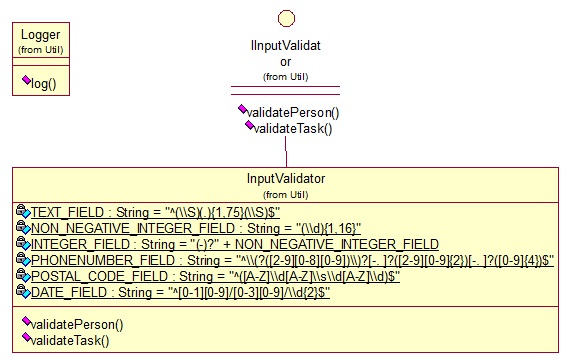
\includegraphics{diagrams/utils_class_diagram}
\\
This package stores all the utility classes needed in the application. Utility classes are classes that are required in multiple components of the application. It contains the Logger, IInputValidator and InputValidator classes.
\\
\subsubsection{Units Description}
\\
\emph{Logger}\\
Functions:\\
\begin{tabular}{| l | l | l | l |}
\hline
Name & Parameters & Pre-conditions & Post-conditions\\
\hline
\multirow{2}{*}{log} & String className, String log & Requires Nothing & Logs \emph{className} and \emph{log} parameters to console
\\&  & & and passed to the main view
\\
\hline
\end{tabular}
\\
Attributes: \emph{none}
\\
Purpose: Its purpose is to log to console the message provided to it. The advantage of a Logger versus directly outputting to console via \emph{System.out.println()} is that it can easily be extended to log to a file without having to made code chage to anywhere else in the application.
\\
\\
\emph{IInputValidator}\\
Functions:\\
\begin{tabular}{| l | l | l | l |}
\hline
Name & Parameters & Pre-conditions & Post-conditions\\
\hline
\multirow{2}{*}{log} & String className, String log & Requires Nothing & Logs \emph{className} and \emph{log} parameters to console\\ 
			 &  & & and passed to the main view
\\
\hline
\end{tabular}
\\
Attributes: \emph{none}
\\
Purpose: Its purpose is to log to console the message provided to it. The advantage of a Logger versus directly outputting to console via \emph{System.out.println()} is that it can easily be extended to log to a file without having to made code chage to anywhere else in the application.
\\
\\
\emph{IInputValidator}\\
Functions:\\
\begin{tabular}{| l | l | l | l |}
\hline
Name & Parameters & Pre-conditions & Post-conditions\\
\hline
\multirow{2}{*}{view} & String path                                 & Requires that path point & Ensures that the tasks have been\\ 
			 & ArrayList$<$Person$>$ people & to a valid location.          & written to the file pointed to by path.\\ 
                                     & ArrayList$<$Task$>$ tasks       &                             & 
\\
\hline
\end{tabular}\\
Purpose: Describe the interface for dumping tasks to a file.

\section{Dynamic Design Scenarios}

\subsection{Add Scenario}
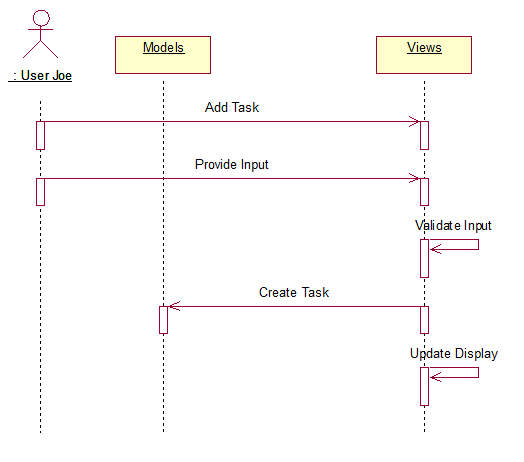
\includegraphics{diagrams/add_sequence_diagram.png}


\subsection{Delete Scenario}
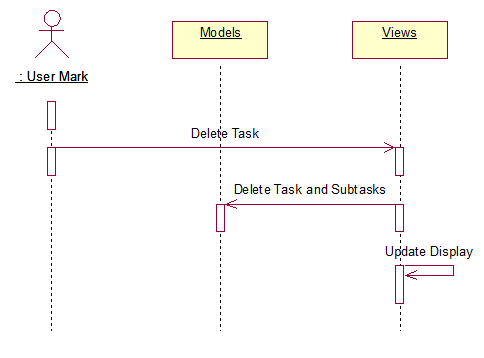
\includegraphics{diagrams/delete_sequence_diagram.png}



\end{document}
